\documentclass[11pt]{article}
\usepackage{makeidx}
\usepackage{multirow}
\usepackage{multicol}
\usepackage[dvipsnames,svgnames,table]{xcolor}
\usepackage{graphicx}
\usepackage{epstopdf}
\usepackage[utf8]{inputenc}
\usepackage{ulem}
\usepackage{import}
\usepackage{hyperref}
\usepackage{amsmath}
\usepackage{amssymb}
\usepackage{tikz}
\usepackage[francais]{babel}
\usetikzlibrary{matrix,shapes,arrows,positioning,chains}
\author{Mohamed SANA}
\title{}
\usepackage[paperwidth=595pt,paperheight=841pt,top=49pt,right=70pt,bottom=35pt,left=70pt]{geometry}
\makeatletter
	\newenvironment{indentation}[3]
	{\par\setlength{\parindent}{#3}
	\setlength{\leftmargin}{#1}       \setlength{\rightmargin}{#2}
	\advance\linewidth -\leftmargin       \advance\linewidth -\rightmargin
	\advance\@totalleftmargin\leftmargin  \@setpar{{\@@par}}
	\parshape 1\@totalleftmargin \linewidth\ignorespaces}{\par}
\makeatother 

\begin{document}
\begin{flushright}
Mardi le 31/01/2017\\
\end{flushright}\\
\newline
\newline
\newline
% La table des matières
\part*{\center{ROBOT SUDOKU (SICOM 2A)}}
\textbf{\begin{center}
Par:\\
BOUDIER Baptiste\\
SANA Mohamed\\
GENTIL Kévin\\
BERTRAND Emile\\
*------------------------------------------------*\\
Tuteur: BERTRAND Rivet\\
\end{center}}
*---------------------------------------------------------------------------------------------------------------------*\\

\newline
\newline
\newline
\tableofcontents
\newpage
\part*{INTRODUCTION}

Ce projet a pour but la réalisation d'un robot autonome capable d'analyser et de résoudre des grilles de Sudoku. Ce robot, basique, de type table traçante devra être en mesure d'acquérir une image de la grille de Sudoku à résoudre, puis procéder à l'analyse de cette image pour y détecter la grille et procéder à sa résolution mathématique. Une fois résolue, le robot devra alors  compléter la grille de Sudoku et tout ceci de façon autonome.  

\section{Cahier des Charges}
\textbf{Cadre du projet :}\\
Notre projet est de construire un robot pouvant résoudre, puis compléter une grille de Sudoku de façon autonome. \\
Pour l'instant, nous avons déjà le corps du robot et il nous reste toute la partie programmation et quelques améliorations de la mécanique et de l'électronique.\\

\textbf{Attentes des utilisateurs :}\\
Le robot doit pouvoir résoudre et remplir la grille quelque soit l'orientation et la taille de celle-ci. Il devra donc pouvoir adapter sa façon d'écrire au cas par cas.\\

\textbf{Définition des objectifs :}\\
Premièrement, il faut que le robot puisse fonctionner avec une grille de taille fixe,que nous définirons, et avec une orientation sur le plateau connue.\\
Deuxièmement, il faut qu'il puisse s'adapter selon une orientation inconnue (taille standard), puis avec une taille non définie (orientation connue). Enfin, il faut qu'il réussisse avec les deux paramètres inconnus.\\
Le robot ne pourra par contre fonctionner que si la grille de Sudoku ne quitte pas un périmètre de 165x165 mm délimité par un carré bleu sur le plateau. Ce périmètre est imposé par la limitation du champ de vision de la caméra.\\

\textbf{Tests :}\\
La validation du système passe par l'implémentation de plusieurs tests. Ces tests doivent prendre en compte plusieurs grilles de tailles différentes avec des orientations différentes.\\
Toutes ces étapes doivent être faites selon le diagramme de Gantt de la figure ~\ref{gantt}

\part{Résolution de la grille: Boucle ouverte}
Dans cette première partie, aucun asservissement n'est réalisé par rapport aux déplacements des moteurs.
\section{Acquisition et pré-traitement d'images}

Dans cette partie l'objectif est de faire l'acquisition d'une image : la grille de Sudoku placée sur le plateau, et d'y appliquer les premiers traitements. Ces traitements consistent en la détermination le l'emplacement de la grille sur le plateau, son orientation ainsi que l'isolement de la grille afin qu'elle puisse être analysée dans la partie suivante. L'image retournée à l'issue de cette étape est une image binarisée (noir et blanc) où la grille est les chiffres ressortent le mieux possible, le plus proche possible de la grille de Sudoku numérique qui a été imprimée (voir figure ~\ref{ii}). Pour effectuer cette étape on se servira d'un raspberry pi ''2011.12'', de la camera ''Rasperry PI camera Rev 1.3'', du langage python ainsi que que de la librairie Opencv.\\
\begin{figure}[!h]
	\centering
   	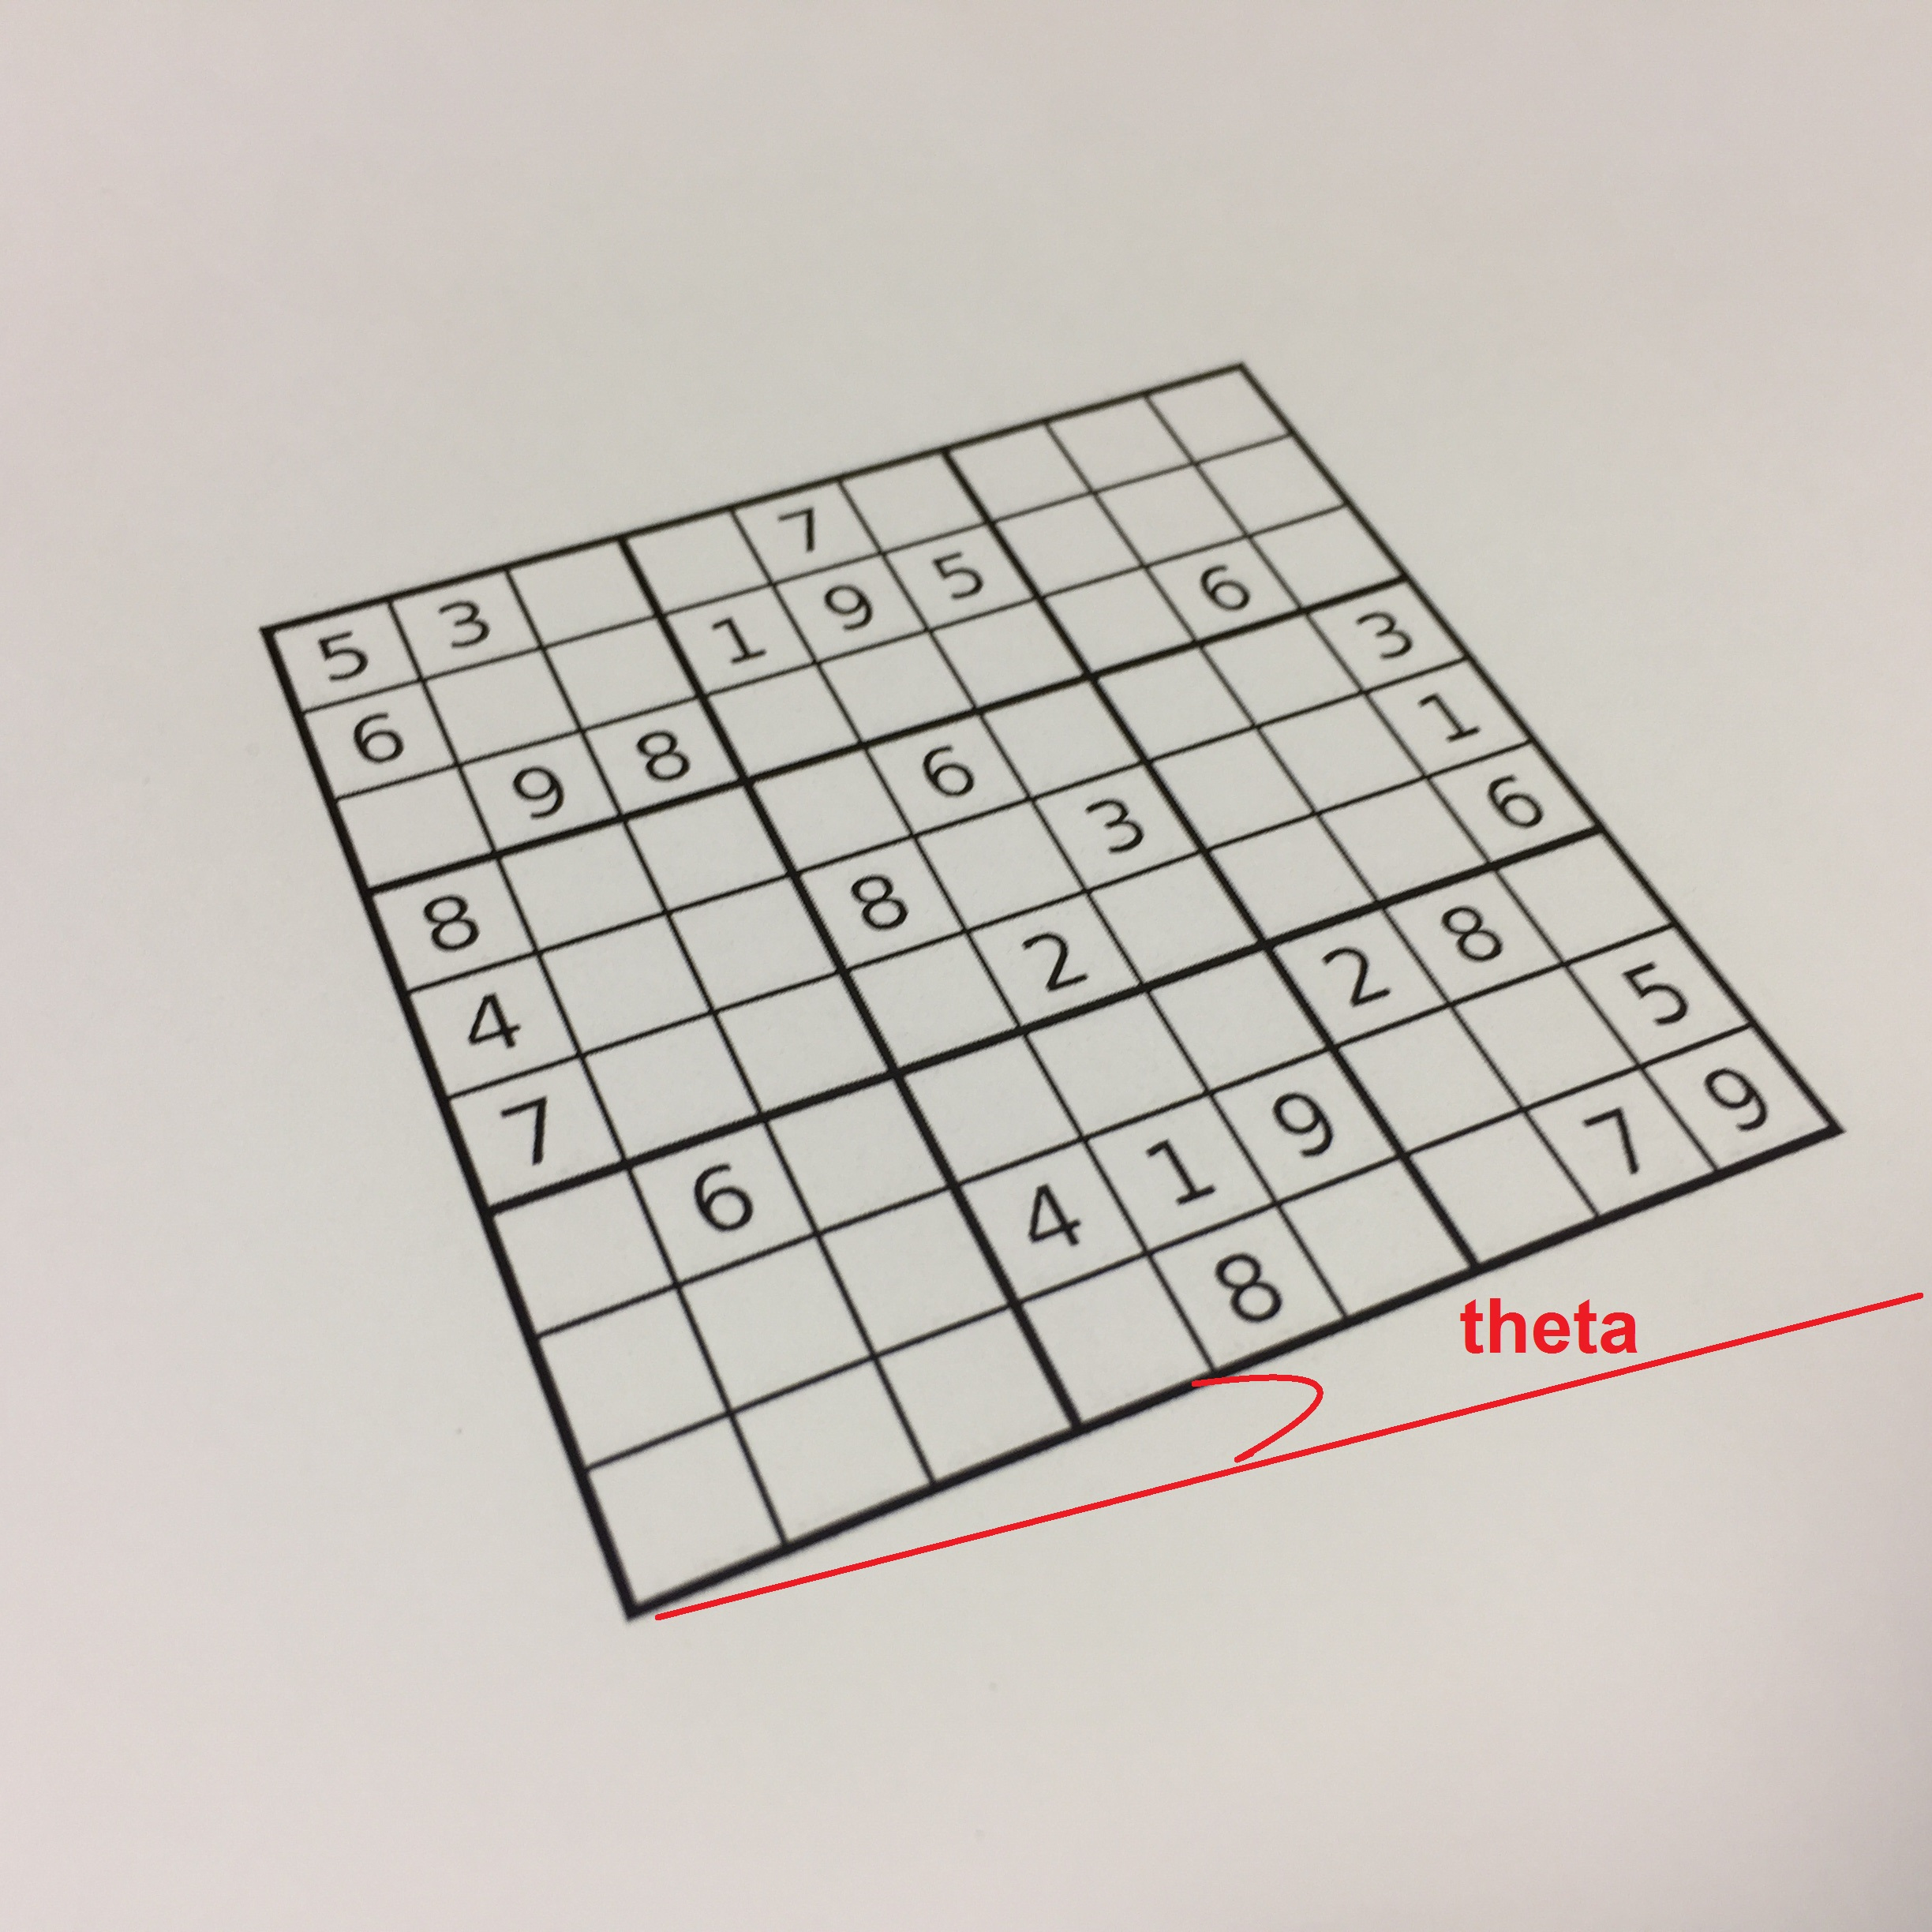
\includegraphics[scale = 0.07]{ii.jpg}
   	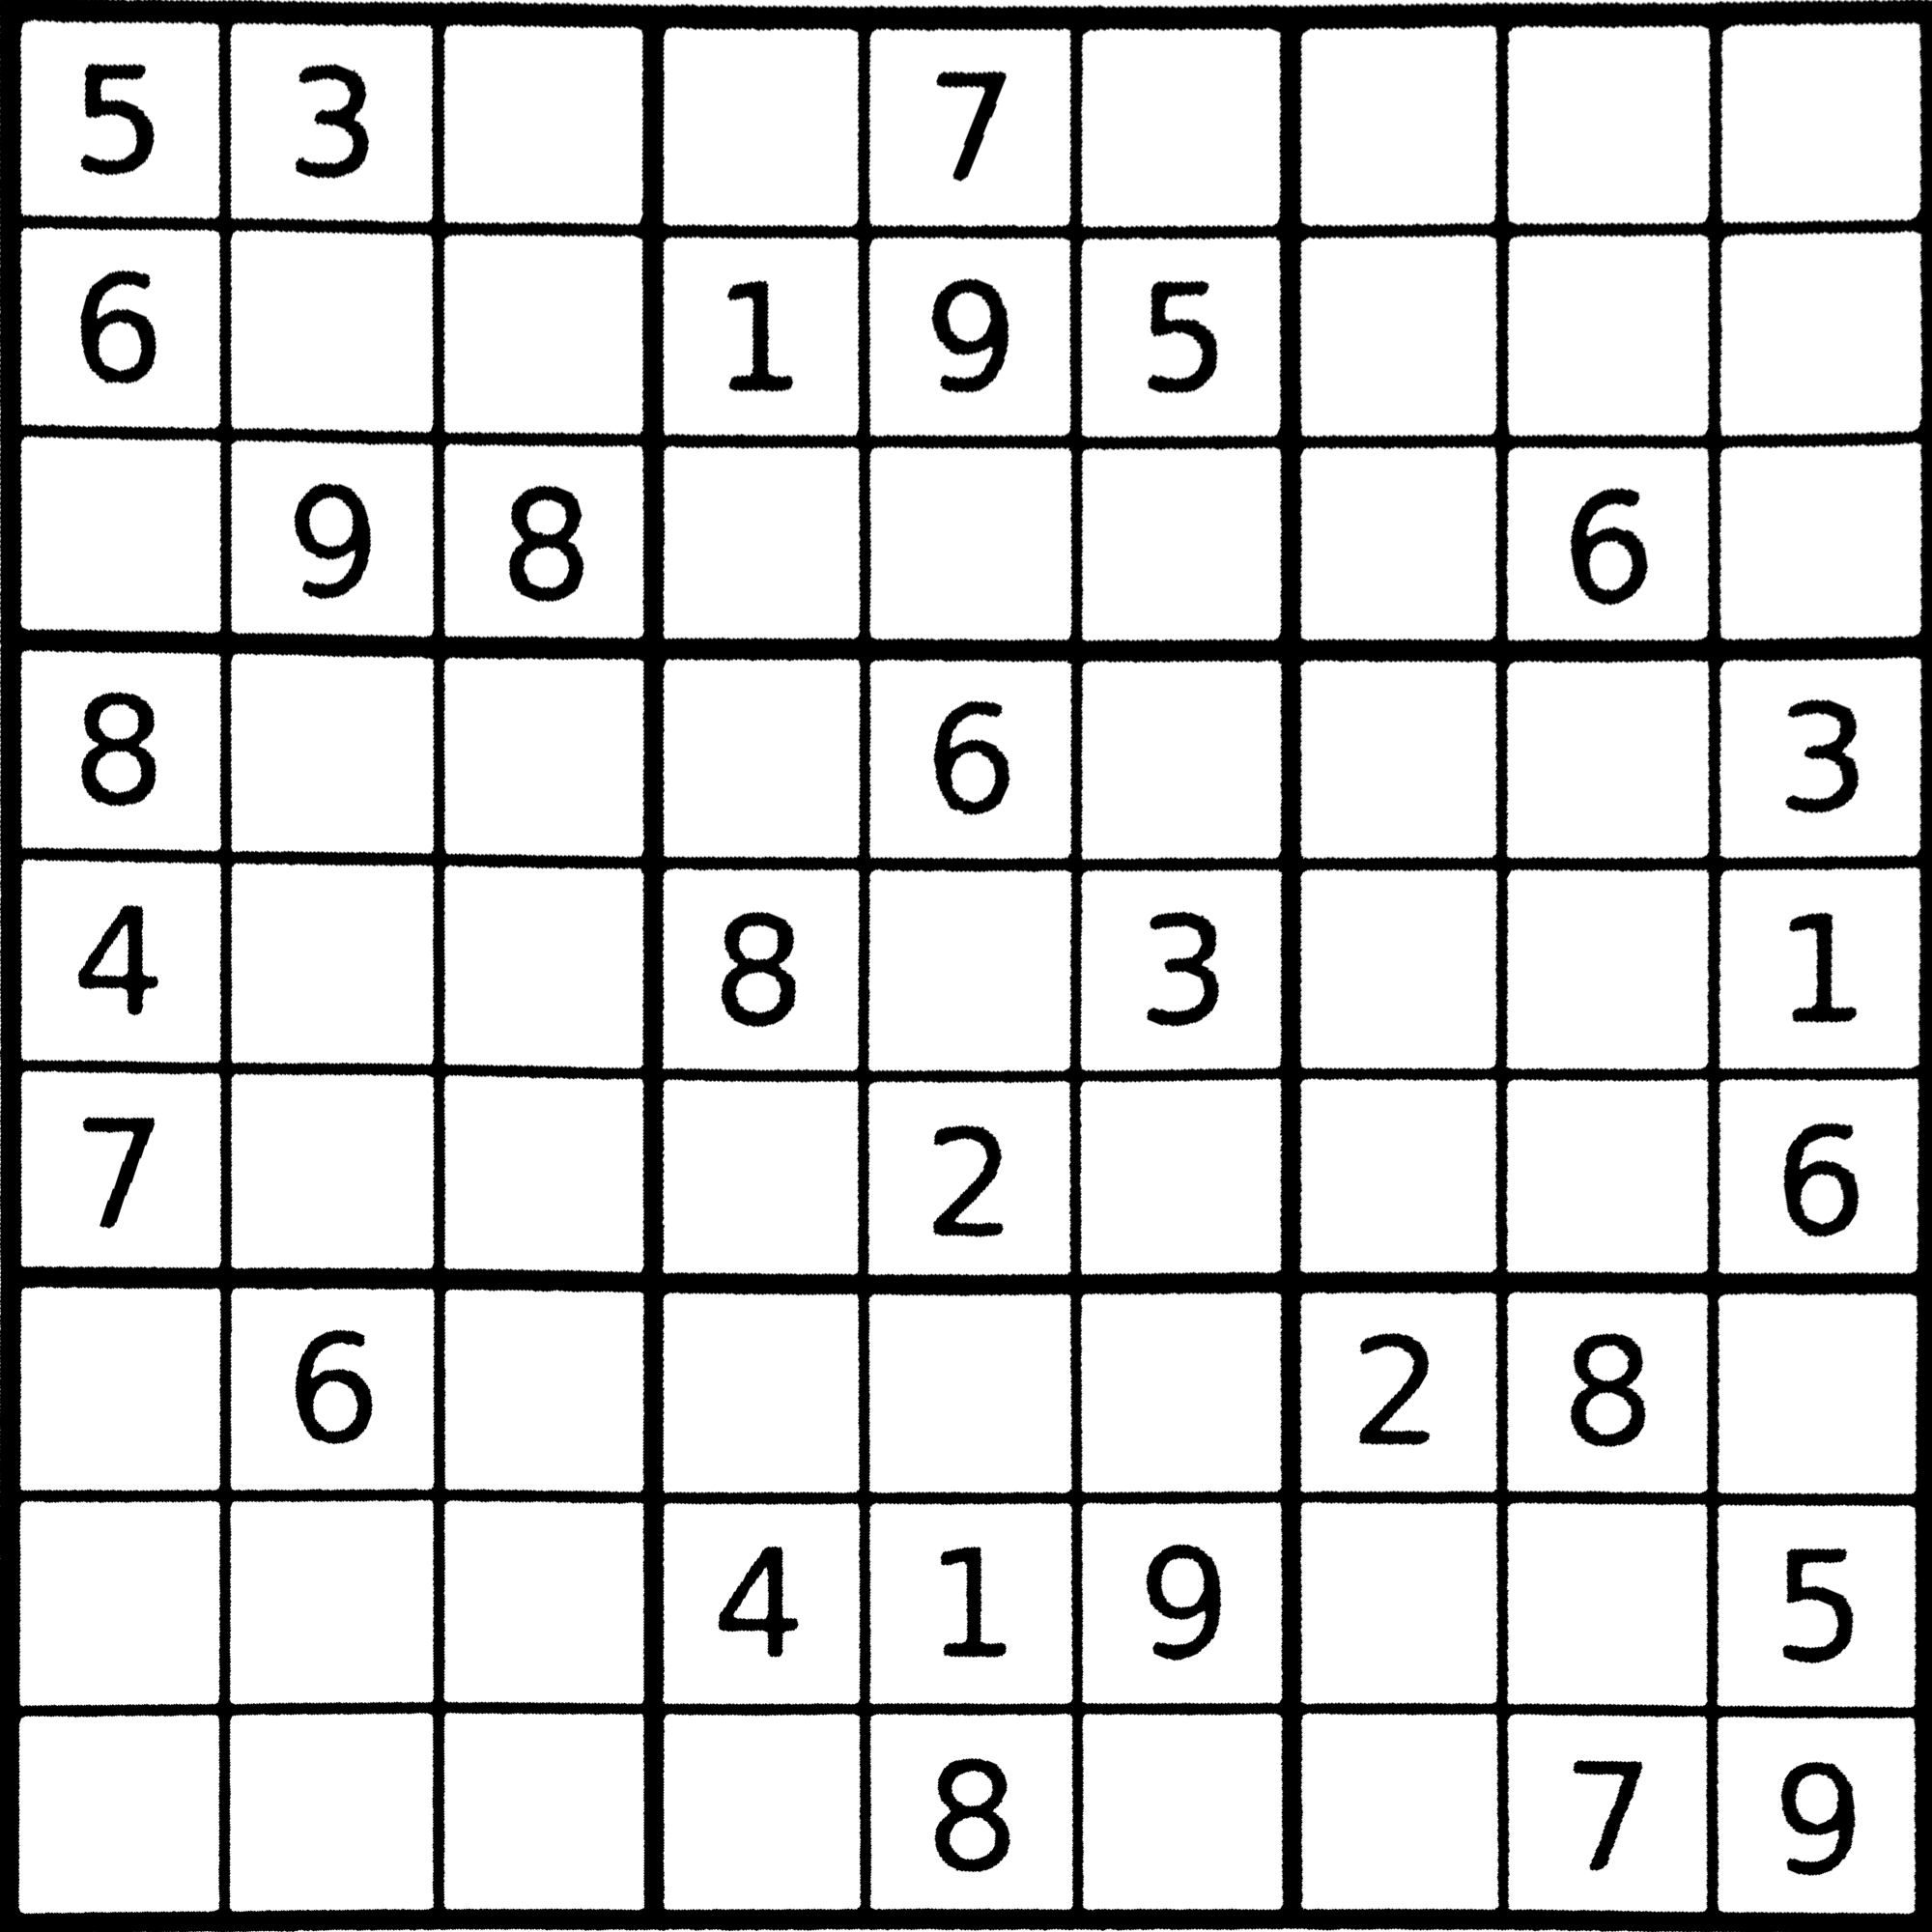
\includegraphics[scale = 0.086]{ii2.png}
   	\caption{\label{ii}wrapping de l'image}
\end{figure}

\section{Détection de la grille et reconnaissance des chiffres}

L'objectif de cette partie, c'est de pouvoir aux moyens de techniques de segmentation d'images, reconnaitre la grille du Sudoku pour en extraire chaque case. Chaque image de case extraite va ensuite subir un certain nombre de traitements, le but étant de pouvoir reconnaitre si celle-ci est vide ou sinon quel chiffre s'y affiche. La valeur de retour de cette étape du traitement est une matrice 9x9 représentant la grille de Sudoku en vu de sa résolution dans l'étape suivante.
	\subsection{Détection de la grille}
Il existe plusieurs techniques permettant de reconnaitre des lignes dans une image. En effectuant ''l'état de l'art'' de ces techniques, 3 méthodes sortent du lots par leur efficacité:
\begin{enumerate}
	\item \textbf{Les projections orthogonales de la grille suivant l'axe x et y:}\\
	L'image de la grille de Sudoku, étant constituée de ligne, les projections de la grille suivant les axes x et y peuvent conduire à des résultats exploitables.\\
	\begin{figure}[!h]
	\centering
   		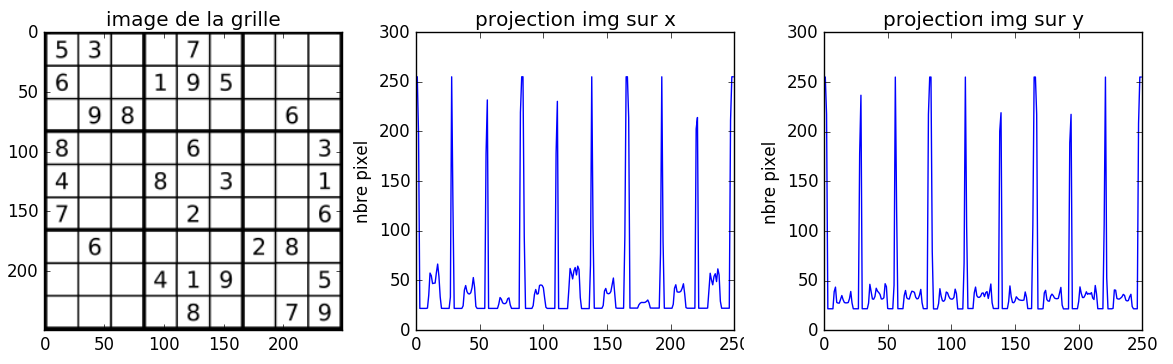
\includegraphics[scale = 0.5]{pp.png}
   		\caption{\label{pp} illustration projection de la grille sur les axes x et y}
	\end{figure}
	On peut ainsi voir sur ces projections ~\ref{pp} , 10 pics reflétant les positions des lignes sur la grille de Sudoku. La mesure de la distance entre-pics pourrait donc permettre de segmenter l'image de Sudoku. 
	\item \textbf{La transformée de Hough:}\\
	Cette méthode se base sur le fait que pour un point de coordonnées (x,y) il existe une infinité de droites passant par ce point mais pour 2 points distincts donnés, il existe une une droite passant par ces 2 points. Pour un point $(x_0,y_0)$ de l'image l'ensemble des droites passants par ce point est donné par l'équation:\\
	$r_\theta = x_0*\cos \theta + y_0*\sin \theta$ (1) \\
	où chaque couple $(r_\theta,\theta)$ représente l'équation d'une droite passant par le point $(x_0,y_0)$.\\
	Ainsi pour $(x_0,y_0)$ donné, on peut représenter le lieu de ces droites (illustration sur la figure ~\ref{hg} en haut à droite). Ce que fait cette méthode c'est représenter pour tous points (x,y) de l'image ce lieu des droites et si par exemple 3 lieux de 3 points donnés se coupent cela implique que ces 3 points sont alignés dans l'image ( illustration faite sur la figure 2 en bas à droite ~\ref{hg}). Par exemple sur notre figure la droite passant par ces trois points est donnée par ses coordonnées polaires (0.96,9.56).\\
	\begin{figure}[!h]
		\centering
   		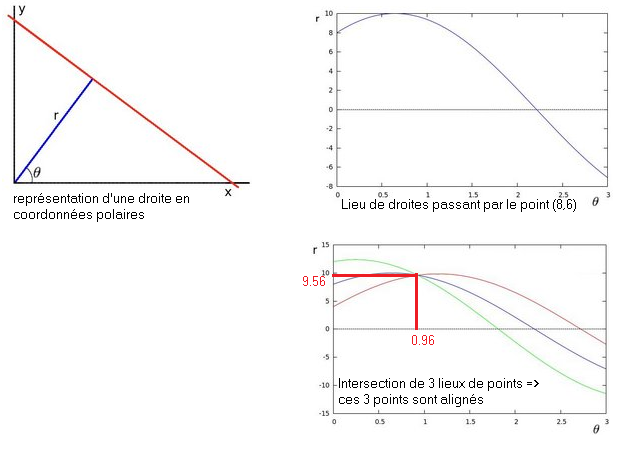
\includegraphics[scale = 0.8]{hg1.png}
   		\caption{\label{hg} illustration transformée de Hough }
	\end{figure}
	
	On voit bien qu'avec cette méthode on pourrait bien détecter la grille de Sudoku, formée  d'ailleurs de ligne. Cependant l'inconvénient de ma méthode c'est que tout ce qui est ligne de pixel sera détecté : il va falloir donc définir ce que nous considérons comme faisant parti de la grille et donc filtrer certaines données!\\
	Exemple d'implémentation de cette méthode que nous avons fait avec la libraire opencv (figure ~\ref{hg1}).
	\begin{figure}[!h]
		\centering
		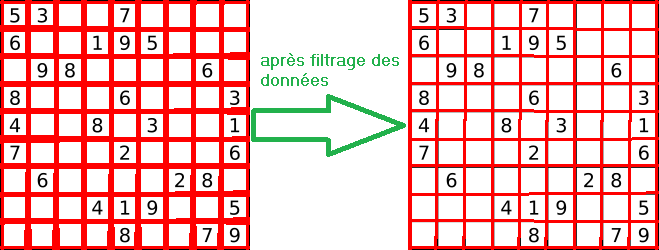
\includegraphics[scale = 0.7]{hough1.png}}
   		\caption{\label{hg1} illustration hough transform sur la grille avec opencv}
	\end{figure}
	\item \textbf{La méthode de la détection des composantes connexes:}\\
	Cette méthode quant à elle permet de détecter les connexités dans l'image. Un pixel est connecté à son voisin si celui-ci est dans le même état que le pixel considéré. Il existe principalement 2 ordres de connexité : 4-connexités (le voisinage du pixel est constitué des 4 plus proches voisin) et 8-connexités( le voisinage du pixel est constitué des 8 plus proches voisin). Cette méthode est très efficace puisque les pixels des lignes de la grille du Sudoku sont aussi connectés.\\
\end{enumerate}
Nous parcourirons toutes ces solutions pour voir les avantages et les inconvénients de chacune d'elle et  choisir la meilleure pour segmenter l'image du Sudoku.
	\subsection{Détection des cases vides}
Une fois l'image segmentée en 9x9 images il va falloir détecter les cases vides du Sudoku. Une case vide est principalement constituée de pixels blancs. Dans la segmentation de l'image, des pixels noirs de la grille peuvent s'y retrouver. Cela veut dire qu'en calculant l'écart type type de chaque image de case, on pourrait trouver un seuil acceptable tel que pour un écart type au dessus de ce seuil, une case sera considérée comme vide.
	
	\subsection{Reconnaissance des chiffres des cases non vides}
Plusieurs techniques de reconnaissance d'images (de chiffres en particulier) existent. Pour notre application, nous avons réffléchi à l'utilisation d'une méthode de reconnaissance par classification et apprentissage de réseaux de neurones ~\ref{rn} . Pour cela la libraire \textbf{tensorflow} de google que nous utiliserons offre un certain nombre de fonctions pour prendre en main ces techniques de classification.

	
 %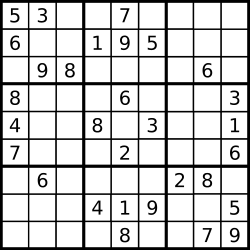
\includegraphics[scale = 0.45]{sud1.png}
 \begin{figure}[!h]
 \centering
\pagestyle{empty}
\def\layersep{2.5cm}
\begin{tikzpicture}[shorten >=1pt,->,draw=black!50, node distance=\layersep]
    \tikzstyle{every pin edge}=[<-,shorten <=1pt]
    \tikzstyle{neuron}=[circle,fill=black!25,minimum size=17pt,inner sep=0pt]
    \tikzstyle{input neuron}=[neuron, fill=green!50];
    \tikzstyle{output neuron}=[neuron, fill=red!50];
    \tikzstyle{hidden neuron}=[neuron, fill=blue!50];
    \tikzstyle{annot} = [text width=4em, text centered]


    % Draw the input layer nodes
    \foreach \name / \y in {1,...,4}
    % This is the same as writing \foreach \name / \y in {1/1,2/2,3/3,4/4}
        \node[input neuron, pin=left:Input(pixels des cases) \#\y] (I-\name) at (0,-\y) {};

    % Draw the hidden layer nodes
    \foreach \name / \y in {1,...,5}
        \path[yshift=0.5cm]
            node[hidden neuron] (H-\name) at (\layersep,-\y cm) {};

    % Draw the output layer node
    \node[output neuron,pin={[pin edge={->}]right:Output[matrice du Sudoku]}, right of=H-3] (O) {};

    % Connect every node in the input layer with every node in the
    % hidden layer.
    \foreach \source in {1,...,4}
        \foreach \dest in {1,...,5}
            \path (I-\source) edge (H-\dest);

    % Connect every node in the hidden layer with the output layer
    \foreach \source in {1,...,5}
        \path (H-\source) edge (O);

    % Annotate the layers
    \node[annot,above of=H-1, node distance=1cm] (hl) {Hidden layer};
    \node[annot,left of=hl] {Input layer};
    \node[annot,right of=hl] {Output layer};
\end{tikzpicture}
\caption{\label{rn} illustration réseaux de neurones }
\end{figure}

\section{Résolution de la grille de Sudoku}
On utilise la méthode par listes chaînées, mais simplifiée car python permet une implémentation plus simple de cette méthode. le principe est simple, on remplace les cases vides par une liste possédant l'ensemble des possibilités, puis on réduit ces listes au fur et à mesure jusqu'à n'obtenir plus qu'une seule possibilité.

%% Define block styles
%\tikzset{
%desicion/.style={
%    diamond,
%    draw,
%    text width=4em,
%    text badly centered,
%    inner sep=0pt
%},
%block/.style={
%    rectangle,
%    draw,
%    text width=10em,
%    text centered,
%    rounded corners
%},
%cloud/.style={
%    draw,
%    ellipse,
%    minimum height=2em
%},
%descr/.style={
%    fill=white,
%    inner sep=2.5pt
%},
%connector/.style={
%    -latex,
%    font=\scriptsize
%},
%rectangle connector/.style={
%    connector,
%    to path={(\tikztostart) -- ++(#1,0pt) \tikztonodes |- (\tikztotarget) },
%    pos=0.5
%},
%rectangle connector/.default=-2cm,
%straight connector/.style={
%    connector,
%    to path=--(\tikztotarget) \tikztonodes
%}
%}
%
%\begin{tikzpicture}
%\matrix (m)[matrix of nodes, column  sep=2cm,row  sep=8mm, align=center, nodes={rectangle,draw, anchor=center} ]{
%    |[block]| {Start};               &  \\
%    |[block]| {Assume that $a=c$ the optimilalty cretierin given by }               &                                            \\
%    |[desicion]| {Locally optimal}          &                                             \\
%   |[block]| {Assume that $a=d$ the optimilalty cretierin given by}    &                                             \\
%    |[desicion]| {Locally optimal}         &                                             \\
%         |[block]| {Assume that $a=e$ the optimilalty cretierin given by}    &                                             \\
%            |[desicion]| {Locally optimal}         &                                             \\
%                 |[block]| {Assume that $a=f$ the optimilalty cretierin given by}    &                                             \\
%                    |[desicion]| {Locally optimal}         &                                             \\
%                         |[block]| {Assume that $a=k$ the optimilalty cretierin given by}    &                                             \\
%                            |[desicion]| {Locally optimal}         &                                             \\
%    |[block]| {Stop};                           &                                             \\
%};
%\path [>=latex,->] (m-1-1) edge (m-2-1);
%\path [>=latex,->] (m-2-1) edge (m-3-1);
%\path [>=latex,->] (m-3-1) edge (m-4-1);
%\path [>=latex,->] (m-4-1) edge (m-5-1);
%\path [>=latex,->] (m-5-1) edge (m-6-1);
%\path [>=latex,->] (m-6-1) edge (m-7-1);
%\path [>=latex,->] (m-7-1) edge (m-8-1);
%\path [>=latex,->] (m-8-1) edge (m-9-1);
%\path [>=latex,->] (m-9-1) edge (m-10-1);
%\path [>=latex,->] (m-10-1) edge (m-11-1);
%\path [>=latex,->] (m-11-1) edge (m-12-1);
%
%\end{tikzpicture}


\section{\'{E}lectronique et contrôle du déplacement des moteurs}
Le contrôle des moteurs se fera avec la carte Raspberry Pi et non plus avec l'Arduino pour une facilité de la gestion du programme.
Même si la Raspberry Pi n'a pas de protection sur ses entrées/sorties, nous avons pas besoin d’optocoupleur car les seules entrées sont des capteurs de fin de course (il ne faut pas oublier les résistances de protection). Les sorties sont reliées au drivers des moteurs et au servomoteur.
Il y a besoin d'une alimentation de 2.8V (tension nominale) pour les moteurs (utilisation d'un régulateur de tension à partir du 5V de la Raspberry Pi).
Cependant les moteurs peuvent demander jusqu'à 1.68A et les drivers n'en fournissent que 1.2A mais peuvent supporter jusqu'à 2A pendant 20 ms or nous avons remarqué à l'oscilloscope que l'on avait des pics de 2A inférieur à 20 ms.\\

Mise en place de deux ou trois leds pour renseigner l'état de la résolution et de l'écriture du Sudoku.\\

Il faut créer des fonctions en python pour contrôler les moteurs, le servomoteur,et les leds à définir suivant les étapes de réalisation dans le software. La mise en place de l'automatisation de l'écriture des chiffres avec la camera qui asservit la position du stylo sera effectuée si tout le reste du projet fonctionne. En attendant, le déplacement de la grille et du stylo sera réalisé en comptant le nombre pas du moteur (fonction du déplacement de la table ou du stylo). Il faut positionner le stylo dans le coin inférieur gauche (ou un autre) d'une case puis appeler une fonction d'écriture d'un chiffre. La création des fonctions en python de l'écriture des chiffres aura en entrée l'angle de la feuille, la dimension d'un côté d'une case ( pour la taille du chiffre). En sortie ces fonctions appelleront directement les fonctions de déplacement des moteurs et du servomoteur.

\part{Résolution de la grille: Boucle fermée}

Dans une deuxième partie, l'objectif du projet sera de réaliser tout le traitement en boucle fermée. En effet dans la première partie le Robot complète la grille ''à l'aveugle'' moyennant les estimations de la position et de chaque case de la grille faite dans la partie pré-traitement. Seulement ces estimations ne sont pas toujours bonnes: on peut écrire de travers. L'idée est de pouvoir, grâce à la caméra, asservir le déplacement des moteurs pour compléter la grille afin d'avoir une meilleur précision d'écriture.\\

\item
\textbf{ORGANISATION DE L'ÉQUIPE}\\
\\
Acquisition et pré-traitement : BOUDIER Baptiste\\
Détection de la grille et reconnaissance des chiffres : SANA Mohamed\\
Résolution du Sudoku + mécanique : GENTIL Kévin\\
Électronique et Contrôle des moteurs : BERTRAND Emile\\
Le diagramme de Gantt de la figure ~\ref{gantt} montre le déroulement du projet.\\

\item
\textbf{Composants, matériels et logiciels utilisés}\\
Toute la programmation se fera avec le langage \textbf{Python} et les libraires suivantes:
\begin{itemize}
\item{Opencv} pour le traitement d'image
\item{Numpy} pour les calculs matriciels
\item{Matplolib} pour l'affichage des courbes et graphes
\item{Tensorflow} pour la classification et la reconnaissance des chiffres
\item{Pycam} pour la gestion de la camera de la Raspbery py
\end{itemize}
\item
Supports matériels:
\begin{itemize}
\item{Raspberry Py}
\item{Arduino}
\item{Moteurs pas à pas et leurs drivers + servomoteurs}
\item{Capteurs de fin de course + régulateurs de tension}
\end{itemize}
\newline
\item
\textbf{Commandes projets}\\
Convertisseur HDMI male VGA femelle (réf: 778-1882) prix: 22.47 euros, chez RS PRO\\
\newpage
\item
\textbf{BIBLIOGRAPHIE}\\
\item
Résolution Sudoku : \url{http://www-ljk.imag.fr/membres/Jerome.Lelong/fichiers/Ensta/sudoku.pdf}\\
Reconnaissance et capture d'images de documents :  \url{https://tel.archives-ouvertes.fr/tel-00821889/document}\\
\url{https://web.stanford.edu/class/ee368/Project_Spring_1415/Reports/Wang.pdf}\\
\url{http://docs.opencv.org/3.0-beta/modules/imgproc/doc/feature_detection.html?highlight=houghline#cv2.HoughLines}\\

\begin{figure}[!h]
	\centering
   	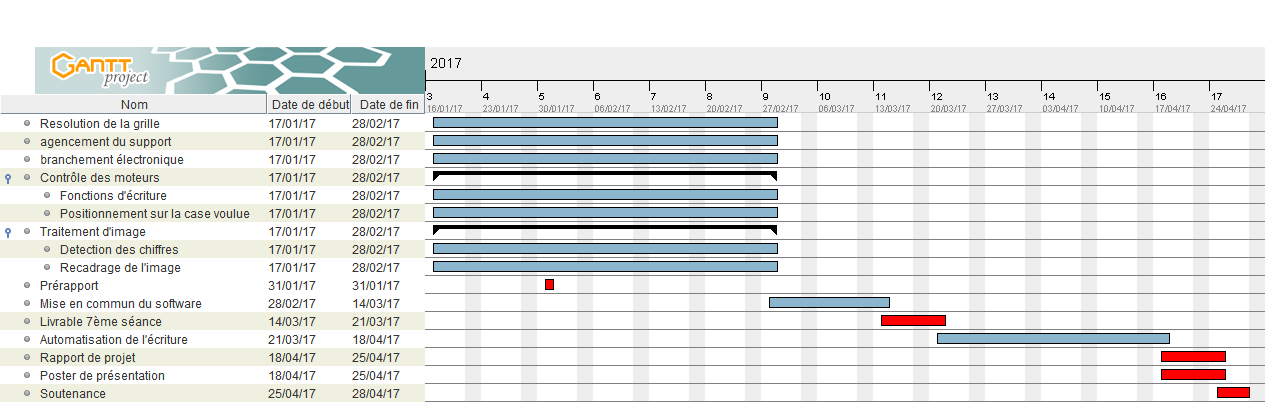
\includegraphics[scale = 0.38]{gantt.png}
   	\caption{\label{gantt} diagramme de Gantt }
\end{figure}


\end{document}
